% \chapter*[Introdução]{Introdução}
% \addcontentsline{toc}{chapter}{Introdução}

% \chapter{Fundamentos Teóricos}

\section{Máquinas de fluxo}

	Máquinas de fluxo são caracterizadas por ser um transformador de energia, em que necessariamente uma das formas de energia é o trabalho mecânico, e a outra é energia de fluido \cite{maq_fluidos_henn}. Quando esse fluido passa por um elemento rotativo, ocorre a transformação de energias. Se a máquina de fluxo recebe trabalho mecânico e o transforma em energia de fluido, chamamos de máquinas de fluxo geradora, pois a energia do fluido aumenta. Desse tipo, são caracterizados as bombas centrífugas e ventiladores. Se a máquina de fluxo recebe energia de fluido e o transforma em trabalho mecânico, chamamos de máquinas de fluxo motora. Desse tipo, são exemplos as turbinas hidráulicas e turbinas a vapor, que será o foco desse trabalho.

\subsection{Elementos fundamentais da máquina de fluxo}

    Para cada máquina de fluxo, existem diversos elementos que a compõem e não será tratado aqui todos eles, mas sim os fundamentais para o funcionamento da máquina. Como o rotor (elemento rotativo) e o sistema diretor.

	Rotor é o elemento rotativo principal de uma máquina de fluxo, é onde ocorre a transformação de energia mecânica em energia de fluido ou vice-versa. É composto por um certo número de pás giratórias que dividem o espaço ocupado em canais, por onde circula o fluido de trabalho, conforme mostrado na \autoref{fig1:rotor_bomba}.

    \begin{figure}[htb]
        \centering
        \caption {\label {fig1:rotor_bomba} Rotor de uma bomba fluxo semi-axial ou fluxo misto}
        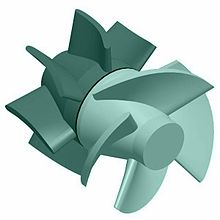
\includegraphics[scale=0.65]{images/fig1.png}
        \legend{Fonte: Wikipédia \cite{wiki_bomba_axial}}
        % \legend{Fonte: Wikipédia \footnote{Bombas Axiais}}
    \end{figure}


    Já o sistema diretor, tem como função, coletar o fluido e dirigi-lo para um caminho determinado. No caso das bombas centrífugas, o sistema diretor de saída é simplesmente um difusor, que transforma parte da energia de velocidade em energia de pressão. Já nas turbinas, o sistema diretor é fundamentalmente um injetor, conforma mostrado na \autoref{fig2:sist_diretor_pelton}, que transforma parte da energia de pressão em energia de velocidade.

    \begin{figure}[htb]
        \centering
        \caption {\label {fig2:sist_diretor_pelton} Sistema diretor de uma turbina hidráulica do tipo Pelton}
        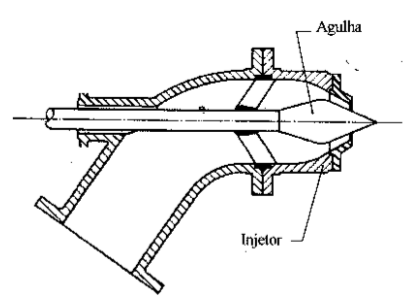
\includegraphics[scale=0.5]{images/fig2.png}
        \legend{Fonte: Máquinas de Fluidos \cite{maq_fluidos_henn}}
    \end{figure}

\subsection{Tipos de Turbinas Hidráulicas}

% \subsubsection{Turbina tipo Francis}

A \textbf{turbina Francis}, é uma turbina hidráulica que foi concebida por Jean-Victor Poncelet por volta de 1820 e aperfeiçoado pelo engenheiro norte-americano James B. Francis \cite{turbina_francis}. Ela se comporta com o fluxo radial de fora para dentro, conforme pode ser visto na Figura \ref{fig3:turbina_francis}.

    \begin{figure}[htb]
        \centering
        \caption {\label{fig3:turbina_francis} Ilustração de uma turbina Francis}
        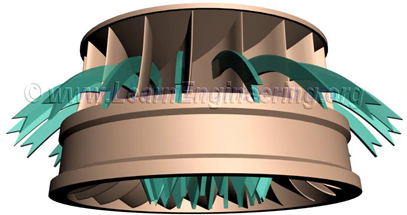
\includegraphics[scale=0.8]{images/fig3.png}
        \legend{Fonte: Learn Engineering \cite{francis_turbine}}
    \end{figure}

    É uma das turbinas mais utilizadas na produção de energia elétrica devido ao seu alto grau de eficiência em um grande ramo de operações. O \textit{head} pode variar de 45 a 400 m, e a vazão de 10 a 700 $m^3/s$. \cite{francis_turbine}

% \subsubsection{Turbina tipo Kaplan}

    A \textbf{turbina Kaplan} é uma turbina hidráulica, inventada por Victor Kaplan. Foi uma evolução da turbina Francis para ter um melhor rendimento com quedas menores. Ela foi projetada para operar com quedas até de 60m, normalmente utilizada entre 2 a 25 e com alta vazão, entre 70 a 800 $m^3/s$. A única diferença entre a turbina Kaplan e a Francis, é o rotor. O rotor da Kaplan se assemelha a um propulsor de navio, conforme pode ser visto na  \autoref{fig4:turbina_kaplan}.

    \begin{figure}[htb]
        \centering
        \caption {\label {fig4:turbina_kaplan} Turbina Kaplan depois de 61 anos de uso. }
        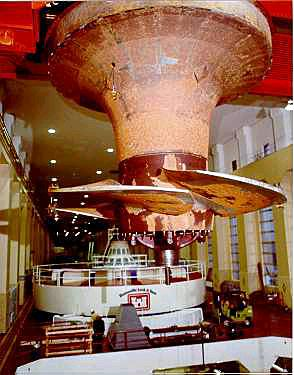
\includegraphics[scale=0.6]{images/fig4.jpg}
        \legend{Fonte: Wikipedia \cite{turbina_kaplan}}
    \end{figure}

% \subsubsection{Turbina tipo Pelton}


    A \textbf{Turbina Pelton} é uma turbina de ação, isto é, funciona à pressão atmosférica, são adequadas para alto \textit{head}, variando entre 350 $m$ até 1100 $m$ e baixa vazão \cite{pelton_turbine}. Foi inventada por Lester Allan Pelton na década de 1870 \cite{turbina_pelton}.

    \begin{figure}[htb]
        \centering
        \caption {\label{fig5:turbina_pelton} Funcionamento da turbina Pelton}
        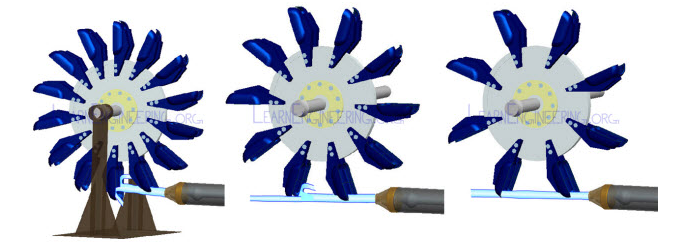
\includegraphics[scale=0.5]{images/fig5.png}
        \legend{Fonte: Learn Engineering \cite{pelton_turbine}.}
    \end{figure}

    É constituída por uma roda, com um ou mais injectores e pás giratórias em forma de dupla concha conforme pode ser visto na \autoref{fig5:turbina_pelton}. Basicamente a turbina Pelton transforma a energia de pressão proveniente do jato de água em alta velocidade em energia de cinética, pois quando o jato incide na dupla concha da turbina Pelton, produz uma força impulsiva que a turbina se movimenta. O eixo rotativo executa um gerador que produz eletricidade.

% \subsection{Potência efetiva de uma turbina hidráulica}
%
%     Sabe-se que potência é o trabalho realizado por uma força na unidade de tempo, para as máquinas hidráulicas a potência efetiva será o produto do peso do fluido que escoa pela máquina, na unidade de tempo pela altura de queda, assim pode-se escrever:
%
%     \begin{equation} \label{eq-potencia}
%         P_e = \rho \, . \,  Q \, . \, Y \, . \, \eta_t
%     \end{equation}
%
%     Onde $\rho$ é a massa específica do fluido, $Q$ a vazão que passa pela máquina, $Y$ o salto energético da máquina e $\eta_t$ o rendimento total da máquina.


\subsection{Campo de Aplicação}

    \begin{figure}[htb]
        \centering
        \caption{\label{fig-camp} Campo de aplicação}
        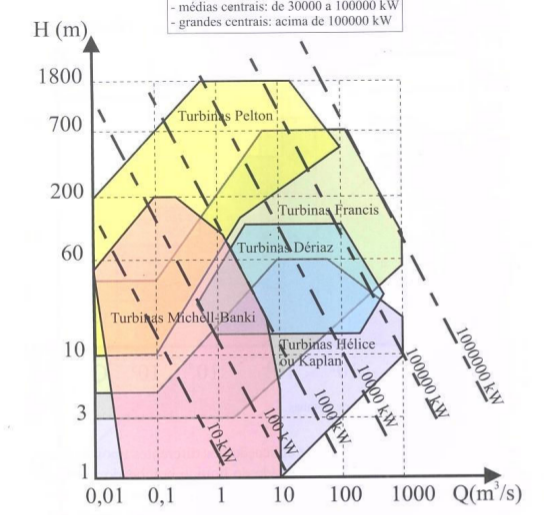
\includegraphics[scale=0.5]{images/campo_de_aplicacao.png}
        \legend{Fonte: Máquinas de Fluidos  \cite{maq_fluidos_henn}.}
    \end{figure}

    Para o ramo das turbinas, existem áreas de superposição entre os campos de aplicação dos diferentes tipos de turbinas, levando em consideração a altura de queda, vazão e a potência. A \autoref{fig-camp} releva predominância em certas áreas de aplicação, como por exemplo de elevada altura de queda e baixa vazão, a turbina Pelton se destaca. Enquanto para grandes vazões e pequena altura de queda a Kaplan se destaca.

\section{Triangulo de Velocidades}

    Um dos conceitos-chave em máquinas de fluxo é entender como o escoamento aparece do ponto de visto do elemento rotativo. Uma vez entendido isso, o entendimento da máquinas de fluxo se torna relativamente mais fácil. Observar a velocidade do escoamento a partir do ponto de vista do rotor em movimento é chamado de \textit{velocidade relativa da corrente fluida} ($\vec{w}$) e a velocidade do escoamento do ponto de vista do observador estacionário é chamado de \textit{velocidade absoluta da corrente fluida} ($\vec{c}$).


    % \begin{figure}[htb]
    %     \centering
    %     \caption {\label{fig7:2motion} Triângulo de velocidades (analogia com o movimento das partículas de água da chuva)}
    %     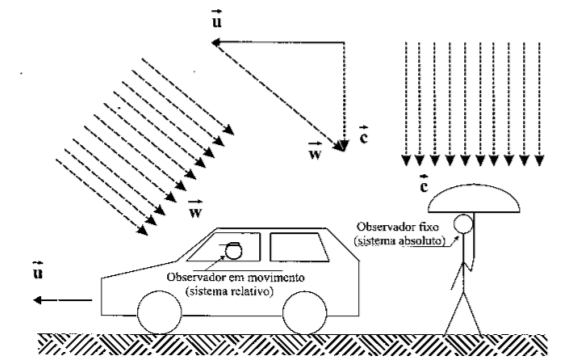
\includegraphics[scale=0.6]{images/fig7.png}
    %     \legend{Fonte: Máquinas de Fluidos  \cite{maq_fluidos_henn}.}
    % \end{figure}
    %
    % Na \autoref{fig7:2motion}, observa-se soma vetorial para o triangulo de velocidades da água da chuva com um carro em movimento, portanto se o observador está em  movimento (como é o caso do elemento rotativo nas máquinas de fluxo), com velocidade $\vec{u}$ e a chuva com a velocidade absoluta da corrente fluida $\vec{c}$, e a soma vetorial dessas velocidades será a velocidade relativa da corrente fluida $\vec{w}$ em relação ao observador em movimento.
    %
    % Nas máquinas de fluxo, o triangulo de velocidades ocorre de forma semelhante conforme demostrado acima.
    A \autoref{fig8:tri_vel} representa o corte segundo um plano meridiano que passa pelo eixo do rotor e pelo corte segundo um plano perpendicular ao eixo do rotor de uma corrente fluida que circula através do rotor de um ventilador (máquina geradora de fluxo).

    \noindent
    Em um ponto qualquer do rotor, denomina-se: \\
        $\vec{u}$ = \textbf{velocidade tangencial} do referido ponto do rotor; \\
        $\vec{c}$ = \textbf{velocidade absoluta da corrente fluida}; \\
        $\vec{w}$ = \textbf{velocidade relativa da corrente fluida}; \\
        $\alpha$ = ângulo que formam os sentidos positivos de $\vec{u}$ e $\vec{c}$ ; \\
        $\beta$ = ângulo que formam o sentido de $\vec{w}$ com o negativo de $\vec{u}$

    \begin{figure}[htb]
        \centering
        \caption {\label{fig8:tri_vel} Escoamento através do rotor de um ventilador centrífugo (máquina de fluxo geradora)}
        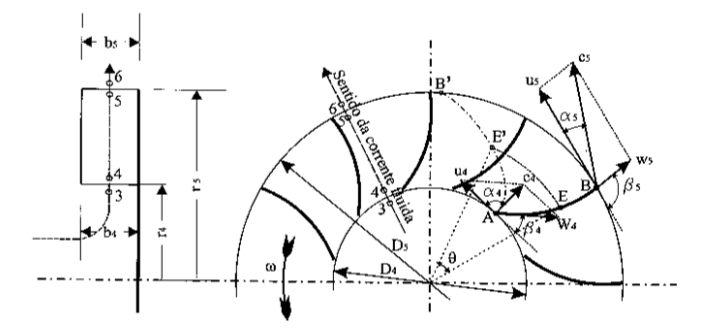
\includegraphics[scale=0.65]{images/fig8.png}
        \legend{Fonte: Máquinas de Fluidos  \cite{maq_fluidos_henn}.}
    \end{figure}

    \noindent
        A estes vetores e suas componentes atribuem-se os seguintes índices: \\
        \textbf{3} = um ponto na corrente de entrada não perturbada, situado imediatamente antes da \textbf{entrada} do rotor; \\
        \textbf{4} = um ponto situado imediatamente depois da entrada do rotor, portanto, já no espaço entre as pás giratórias; \\
        \textbf{5} = um ponto situado imediatamente antes da \textbf{saída} do rotor, portanto, ainda no espaço entre as pás giratórias; \\
        \textbf{6} = um ponto  na corrente de saída não perturbada, situado imediatamente depois da saída do canal móvel.

        Considere a \autoref{fig8:tri_vel} um rotor radial constituído de um número infinito de pás, de espessura infinitesimal, separadas por canais infinitesimais também. Isso implica que o fluxo através dele será unidimensional e que a corrente fluida será tangente às pás do rotor, em todos os seus pontos.

        As pás são construídas de modo inicial para que não haja mudança brusca de direção e perdas de energias devido a formação de vórtices por exemplo. No ponto \textit{A} temos o triângulo de velocidades da corrente fluida imediatamente após a entrada do rotor, e no ponto \textit{B} o triângulo de velocidades da corrente fluida imediatamente antes da saída do rotor. A \autoref{fig9:tri_vel} representa um triângulo de velocidades genérico, em que se faz a decomposição dos vetores $\vec{c}$ e $\vec{w}$ em componentes meridianas com o índice \textit{m} e em componentes tangenciais com o índice \textit{u}.

    \begin{figure}[htb]
        \centering
        \caption {\label {fig9:tri_vel} Triangulo de velocidades genérico }
        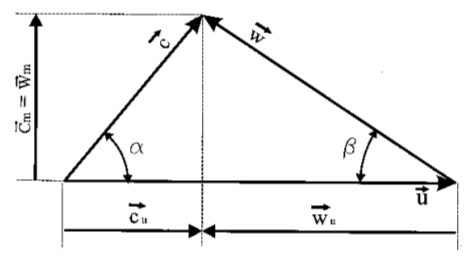
\includegraphics[scale=0.65]{images/fig9.png}
        \legend{Fonte: Máquinas de fluidos  \cite{maq_fluidos_henn}}
    \end{figure}

    A componente tangencial está vinculada com a energia intercambiada entre o rotor e o fluido, enquanto a componente meridiana, de módulo $\vec{c}_m$ está vinculada à vazão da máquina, por meio da equação da continuidade: Q = A $c_m$.

% \section{Máquinas Semelhantes}
%
% \chapter{Motivação}
%
% \section{Exemplos de modelo reduzido}
%
% \section{Projeto}
%
% \chapter{Cálculo e Explicações}

% \chapter*[Considerações Finais]{Considerações Finais}
% \addcontentsline{toc}{chapter}{Considerações Finais}
